\chapter{Physical Model of Volcanic Plume} \label{chapter:physics-model}
\section{Introduction}
The volcanic plume development process is multiphase turbulent mixing flow accompanied by microphysics. Ignoring less dominant physical effects would reduce number of phases, number of governing equations, terms in governing equations making software development numerically, computationally and practically more feasible. Based on assumptions regarding the physics involved in plume development process, a complete mathematical descriptions of the problem, written in form of a set of partial differential equations (PDEs), initial conditions and boundary conditions, are obtained. These PDEs, also named as governing equations, originate naturally
from constitutive relationships and the application of the fundamental laws of conservation of mass, Newton’s Second Law and the law of conservation of energy. Eigenstructure of the governing equations are also analyzed in this chapter which is essential for the implementation of advanced numerical methods, such as GSPH and RSPH.

\section{Volcanic plume development}
During an explosive eruption, a volcanic jet erupts out from a vent with a speed of several tens to more than 150 meters per second, driven by expanding gas. The jet is initially denser than the surrounding atmosphere and begins to decelerate through negative buoyancy and turbulent interaction with surrounding air. Cauliflower-like vortices are generated along jet margins, within which process, air is entrained and heated up, reducing the bulk density of the entire jet, in many cases, to less than that of the surrounding atmosphere. Once it becomes buoyant, such a jet develops into a plinian or subplinian plume, rising up to several kilometers to tens of kilometers until its heat is exhausted. Jets that lose their momentum before becoming buoyant collapse back onto the ground and transform into pyroclastic flows, surges and ignimbrites. During the process of plume rising up, relatively larger particles might separate from main stream of the plume, falling down onto the ground and possibly be re-entrained into the plume at a lower height \citep{ernst1996sedimentation}. Within this process, erupted vapor condenses to liquid (droplet) and even further to ice. Latent heat released from phase change of erupted vapor  further heats up entrained air and further dilutes the bulk density. The entrained vapor might also experience a similar process and impact plume development. Particle aggregation processes \citep{carey1982influence,taddeucci2011aggregation}, either due to presence of liquid water, resulting from particle collision or driven by electrostatic forces might occur inside plume and thereby affect the sedimentation. 

All in all, the process of plume development is  essentially a multiphase turbulent mixing process coupled with heat transfer and other microphysical and chemical reactions.

As an initial effort on exploiting the feasibility and advantage of SPH in plume modeling, our model is designed to describe an injection of well mixed solid and volcanic gas from a circular vent above a flat surface into a stratified stationary atmosphere following SK-3D \citep{suzuki2005numerical}. In this model, molecular viscosity and heat conduction is neglected since turbulent exchange coefficients are dominant. Erupted material consisting of solid with different size and mixture of gases is assumed to be well mixed and behave like a single phase fluid (phase 2) which is valid for eruptions with fine particles and ash. Air (also a mixture of different gases) is assumed to be another phase (phase 1). Thermodynamic equilibrium is assumed so that no separate energy equation is needed for each phase. As a result, there is only one energy equation for both phases (heat exchange term between different phases does not show up under this assumption). Dynamic equilibrium is assumed so that no separate momentum equation is needed for each phase. As a result, there is only one vector momentum equation for both phases (drag force term does not show up with this assumption). 

Because of the above assumptions, all other microphysical processes (such as the phase changes of $HO_2$, aggregation, disaggregation, absorption of gas on the surface of solids, solution of gas into a liquid) and chemical processes are not considered in this model. These ignored microphysics factors would play critical roles under particular eruption conditions. Capturing of these processes needs a more comprehensive model. One critical element in plume development, the effect of wind, is also not yet considered in this model. Introducing wind effects in our model requires dynamic pressure boundary conditions, which requires more numerical effort and algorithm design. To summarize, our model is not valid for eruptions where wind effect plays a significant role in its development, usually refered as a weak plume. Our model also lacks the ability in modeling plumes with large particles or eruptions in which microphysics plays non-ignorable roles, such as an eruption of \textit{El Chich{\'o}n} volcano on April 4th 1982 \citep{sigurdsson19841982, folch2016fplume}. We are focussed here on developing the SPH based methodoloy in the context of the more basic (and more critical) aspects of volcanic plume and therefore devote our effort to this relative simpler model. It is worthwhile to mention here that because SPH is adopted as our numerical method, adding of these physics into our model would require much less work in terms of programming compared to mesh based methods. Since our plan is an open source distribution of the tool we believe some of these enhancements will rapidly ensue with community participation.

\section{Mathematical description}\label{sec:chp2-Mathematical-Description}

The following assumptions are made:
\begin{itemize}
\item Molecular Viscosity is neglected since eddy viscosity due to turbulence is dominant. Such assumption is a common practice when modelling turbulent flow, for which Reynolds number (ration between inertial force and viscous forces) is large.
\item Erupted material consist of solid with different size and mixture of gas (various constituent) is assumed to be well mixed and behave like a single phase fluid (phase 2). Air (also a mixture of different gas) is assumed to be another phase (phase 1).
\item Immediate thermodynamics equilibrium is assumed so that no separate energy equation is needed for each phase. As a result, there is only one energy equation for both phases (Heat transfer term will not show up under this assumption.). 
\item Immediate dynamics equilibrium is assumed so that no separate momentum equation is needed for each phase. As a result, there is only one vector moment equation for both phases (Drag force term will not show up in the equation).
\item Because of above assumptions, all other micro-physics process (like phase change of $H_2O$, aggregation, decomposition, absorption of gas on the surface of solid, solution of gas into the liquid,) and chemical process will not be considered in this model.
\item Assume the effects of wind field is ignorable so that the atmosphere could be treated as stationary. 
\end{itemize}

\subsection{Governing equations}
Based on above assumptions, the governing equations of our model are given as (which is the same as the governing equations of SK-3D \citep{suzuki2005numerical}):
\begin{align}
\dfrac{\partial \rho}{\partial t} + \nabla \cdot \left(\rho \textbf{v}\right) = 0 \label{eq:gov-cs-rho} \\
\dfrac{\partial \rho \xi}{\partial t} + \nabla \cdot \left(\rho \xi \textbf{v}\right) = 0 \label{eq:gov-cs-ks}\\
\dfrac{\partial \rho \textbf{v}}{\partial t} + \nabla \cdot \left(\rho \textbf{v} \textbf{v} + p\textbf{I}\right) = \rho \textbf{g} \label{eq:gov-cs-v} \\
\dfrac{\partial \rho E}{\partial t} + \nabla \cdot \left[\left(\rho E + p \right)\textbf{v}\right] = \rho \textbf{g} \cdot\textbf{v} \label{eq:gov-cs-e}
\end{align}
where $\rho$ is the density, $\textbf{v}$ is the velocity, $\xi$ is the mass fraction of ejected material, $\textbf{g}$ is the gravitational acceleration, $\textbf{I}$ is a unit tensor.
$E = e + K $ is the total energy which is a summation of kinetic energy $K$ and internal energy $e$.
An additional equation is required to close the system. In this model, the equation for closing the system is the following EOS (equation of state).
\begin{equation}
p = \left(\gamma_m - 1\right)\rho e \label{eq:EOS}
\end{equation}
where 
\begin{equation}
\gamma_m = R_m/C_{vm} + 1 \label{eq:gov-gm}
\end{equation}
\begin{equation}
R_m = \xi_g R_g + \xi_a R_a  \label{eq:gov-Rm}
\end{equation}
\begin{equation}
C_{vm} = \xi_s C_{vs} + \xi_g C_{vg} + \xi_a C_{va} \label{eq:gov-Cvm}
\end{equation}
\begin{equation}
\xi_a = 1 - \xi \label{eq:gov-na}
\end{equation}
\begin{equation}
\xi_g = \xi \cdot \xi_{g0} \label{eq:gov-ng}
\end{equation}
\begin{equation}
\xi_s = \xi - \xi_g \label{eq:gov-ns}
\end{equation}
where, $C_v$ is the specific heat with constant volume, $R$ is the gas constant. $\xi$ with subscript is the mass fraction of corresponding constituent. The subscript 
$m$ represents mixture of ejected material and air, $s$ represents solid portion in the ejected material, $g$ represents gas portion in the ejected material and $a$ represents air. $\xi_{g0}$ is the mass fraction of vapor in the erupted material.

In mesh based methods, governing equations in Eulerian form, Eq. (\ref{eq:gov-cs-rho}) to Eq. (\ref{eq:gov-cs-e}), are directly discretized. For SPH, governing equations in Lagrange form are needed. By deducting kinetic energy from energy equation, subtracting mass conservation from momentum equation, combining transient term and advection term into material derivative term (For any function $A$, material derivative is defined as $\frac{D A}{Dt} = \frac{\partial A}{\partial t} + \textbf{v} \cdot \nabla A$), the governing equations are put into the final form, in which advection term does not appear explicitly.
\begin{align}
\dfrac{D \rho}{D t} + \rho \nabla \cdot \textbf{v} = 0 \label{eq:gov-nc-rho}\\
\dfrac{D \rho \xi}{D t} + \rho \xi \nabla \cdot \textbf{v} = 0 \label{eq:gov-nc-ks}\\
\dfrac{D \textbf{v}}{D t} + \dfrac{\nabla P}{\rho} =\textbf{g} \label{eq:gov-nc-v}\\
\dfrac{D e}{D t} + \dfrac{P \nabla \cdot \textbf{v}}{\rho} = 0 \label{eq:gov-nc-e}
\end{align}
%Governing equations in Lagrangian form, Eq. (\ref{eq:gov-nc-rho}) to Eq.(\ref{eq:gov-nc-e}), and Eulerian form, Eq. (\ref{eq:gov-cs-rho}) to Eq. (\ref{eq:gov-cs-e}), are a\dfrac{•}{•}ly equivalent, as deriving the Lagrangian form from the Eulerian is purely based on mathematics without any additional physical assumptions.

\subsection{Boundary conditions}
In the current model the initial domain is a box. The boundaries are categorized as the velocity inlet (a circular area at the center of the bottom of the box), wall boundary (box bottom), pressure outlet (other faces of the box).
%probably should add a section to list the input parameters in the verification section

\subsubsection{Velocity inlet}
At the vent, temperature of erupted material $T$, eruption velocity $\textbf{v}$, the mass fraction of vapor in erupted material $\xi_{g0}$ and mass discharge rate $\dot M$ are given. The pressure of erupted material $p$ is assumed to be the same as ambient pressure for pressure-balanced eruption. The radius of vent is determined from $\rho$, $\dot M$ and $\textbf{v}$. Equation (\ref{eq:erupt_bc_rho}) to (\ref{eq:erupt_bc_e}) gives velocity inlet boundary condition wrote in terms of primitive variables.
\begin{align}
\rho =const = p/\left(R_m T\right) \label{eq:erupt_bc_rho} \\
\xi=const=1 \label{eq:erupt_bc_xi}\\
\textbf{v} = const =\{u,v,w\}^T \label{eq:erupt_bc_v}\\
\dfrac{\partial e}{\partial n}=\dot M e /\left(\pi r^2\right) \label{eq:erupt_bc_e}
\end{align} 
where $r$ is the radius of the vent, $n$ is the direction normal to the boundary.

\subsubsection{Non-slip wall boundary}
Velocity is zero for non-slip wall boundary. If we assume the boundary to be adiabatic, heat flux should be zero on the boundary. The flux of mass should also be zero. As a result, internal energy flux, which consists of heat flux and energy flux carried by mass flux, vanishes on the wall boundary. Equation (\ref{eq:wall_bc_rho}) to (\ref{eq:wall_bc_e}) gives no-slip wall boundary condition written in terms of primitive variables.
\begin{align}
\dfrac{\partial \rho}{\partial n} = const = 0\label{eq:wall_bc_rho} \\
\dfrac{\partial \xi}{\partial n} = const = 0 \label{eq:wall_bc_xi}\\ 
\textbf{v} = const =\{0,0,0\}^T \label{eq:wall_bc_v}\\
\dfrac{\partial e }{\partial n} = 0\label{eq:wall_bc_e}
\end{align} 

\subsubsection{Open outlet pressure boundary condition}
The pressure of the surrounding atmosphere is given. Except for the pressure, boundary values for density, velocity, and energy on the outlet should depend on the solution. As we ignore the viscosity, the shear stress is ignored and normal stress (whose magnitude equals to pressure) balances the ambient pressure.
\begin{equation}
p = p_a\left(z\right)  \label{eq:pressure_bc_p} 
\end{equation}

\section{Eigenstructure analysis}
In this section, the governing equations are categorized into two weakly coupled subgroups based on eigenstructure and elementary wave solution analysis. Such simplification is the basis of utilising GSPH formulations and Riemann solvers of Euler equations to solve our governing equation with GSPH.

Eigenstructures of the homogeneous governing equations is analysed to find the eigenvalues and eigenvectors, which is the basis for defining and solving of Riemann problems. In GSPH, only a 1D Reimann problem need to be solved. So we analyse the 1D homogeneous governing equations. 
\begin{align}
\dfrac{\partial \rho}{\partial t} + \dfrac{\partial \rho u} {\partial x}= 0 \label{eq:gov-cs-rho-1d-hom} \\
\dfrac{\partial \rho \xi}{\partial t} + \dfrac{\partial \rho \xi u} {\partial x}= 0 \label{eq:gov-cs-ks-1d-hom}\\
\dfrac{\partial \rho u}{\partial t} + \dfrac{\partial \rho u u} {\partial x} + \dfrac{\partial p} {\partial x}= 0 \label{eq:gov-cs-v-1d-hom} \\
\dfrac{\partial \rho (e+\dfrac{1}{2}u^2)}{\partial t} + \dfrac{\partial \rho u (e+\dfrac{1}{2}u^2) } {\partial x} + \dfrac{\partial pu} {\partial x} = 0 \label{eq:gov-cs-e-1d-hom}
\end{align}
Where the vector velocity $\textbf{v}$ degenerates to a scalar velocity $u$. Equation (\ref{eq:gov-cs-rho-1d-hom}) $\sim$ (\ref{eq:gov-cs-e-1d-hom}) can be written in a more concise form:
\begin{equation}
\textbf{U(x,t)}_t + \textbf{F(\textbf{U}(x, t))}_x = 0
\end{equation}
With primitive variable vector
\begin{equation}
   \textbf{U}=\begin{bmatrix}
         u_1 \\
         u_2 \\
         u_3 \\
         u_4
     \end{bmatrix}
    =\begin{bmatrix}
         \rho \\
         \rho\xi \\
         \rho u   \\
         \rho(e+\frac{1}{2}u^2)
     \end{bmatrix}
\end{equation}
and flux vector: 
\begin{equation}
   \textbf{F}=\begin{bmatrix}
         \rho u \\
         \rho\xi u \\
         \rho u  u + p  \\
         \rho u(e+\frac{1}{2}u^2) + pu
     \end{bmatrix}
\end{equation}

It might facilitate analysis of the eigenstructure if the governing equations are formulated in terms of variables other than conserved quantities. One of the choices is using pressure in place of internal energy and using mass fraction in place of density of phase 2. Based on EOS (Eq. (\ref{eq:EOS})), the new formulation of the governing equations are obtained (see Eq. (\ref{eq:gov-PressForm-rho-1d-hom}) $\sim$ (\ref{eq:gov-PressForm-p-1d-hom}), which we refer as pressure equations in later section).

\begin{eqnarray}
\dfrac{\partial \rho}{\partial t} + u \dfrac{\partial \rho} {\partial x} + \rho \dfrac{\partial u} {\partial x}= 0 \label{eq:gov-PressForm-rho-1d-hom} \\
\dfrac{\partial \xi}{\partial t} + u \dfrac{\partial \xi} {\partial x}= 0 \label{eq:gov-PressForm-ks-1d-hom}\\
\dfrac{\partial u}{\partial t} + u \dfrac{\partial u} {\partial x} + \frac{1}{\rho} \dfrac{\partial p} {\partial x}= 0 \label{eq:gov-PressForm-v-1d-hom} \\
\dfrac{\partial p}{\partial t} + u \dfrac{\partial p} {\partial x} + \gamma_m p \dfrac{\partial u} {\partial x} = 0 \label{eq:gov-PressForm-p-1d-hom}
\end{eqnarray}
With the more concise formulation: 
\begin{equation}
\textbf{W}_t + \textbf{A(\textbf{W})} \textbf{W}_x = 0
\end{equation}
Where primitive variable vector
\begin{equation}
   \textbf{W}=\begin{bmatrix}
         w_1 \\
         w_2 \\
         w_3 \\
         w_4
     \end{bmatrix}
    =\begin{bmatrix}
         \rho \\
         \xi \\
         u   \\
         p
     \end{bmatrix}
\end{equation}
and Jacobian matrix: 
\begin{equation}
   \textbf{A(\textbf{W})}=\begin{bmatrix}
         u & 0 & \rho       & 0 \\
         0 & u & 0          & 0 \\
         0 & 0 & u          &\frac{1}{\rho} \\
         0 & 0 & \gamma_m p & u
     \end{bmatrix}
\end{equation}
The eigenvalues of the Jacobian are: $\lambda_1 = u-c$,  $\lambda_2 = \lambda_3 = u$ and $\lambda_4 = u+c$. Where $c=(\frac{\gamma_m p}{\rho})^{\frac{1}{2}}$ is the sound speed of mixture. The corresponding eigenvectors are: 
\begin{equation}
   k_1 =\begin{bmatrix}
         1 \\
         0 \\
         \frac{-c}{\rho} \\
         c^2
     \end{bmatrix},
   k_2 =\begin{bmatrix}
         1 \\
         0 \\
         0   \\
         0
     \end{bmatrix},
   k_3 =\begin{bmatrix}
         0 \\
         1 \\
         0   \\
         0
     \end{bmatrix},
   k_4 =\begin{bmatrix}
         1 \\
         0 \\
         \frac{c}{\rho} \\
         c^2
     \end{bmatrix}
     \label{eq:eigenvector-pressure}
\end{equation}

It can be proved that the characteristic fields associated with second and third eigenvalues are linear degenerate while the these corresponding to first and forth are genuinely nonlinear. It is obvious that across these two waves associated with $\lambda_2$ and $\lambda_3$, only $\xi$ and $\rho$ changes, which will be proved in later section. Having an additional equation for mass fraction introduces an extra linear degenerate waves.

Based on the relationship between entropy, pressure and density (Eq. (\ref{eq:entropy-p-rho})), the governing equations can be written in term of $\rho	$, $\xi$, $u$, $s$ (the entropy).
\begin{equation}
s=C_v ln(\dfrac{p}{\rho^{\gamma_m}})+C_0 \label{eq:entropy-p-rho}
\end{equation}
Then
\begin{equation}
p=C_1 \rho^{\gamma_m} exp(\frac{s}{C_v})
\end{equation}
With $C_1=exp(-\frac{C_0}{C_v})$.
After lengthy derivation, the last governing equation can be written in terms of entropy and the complete set of governing equations (which will be refered as entropy equations in later sections) are: 
\begin{eqnarray}
\dfrac{\partial \rho}{\partial t} + u \dfrac{\partial \rho} {\partial x} + \rho \dfrac{\partial u} {\partial x}= 0 \label{eq:gov-EntropyForm-rho-1d-hom} \\
\dfrac{\partial \xi}{\partial t} + u \dfrac{\partial \xi} {\partial x}= 0 \label{eq:gov-EntropyForm-ks-1d-hom}\\
\dfrac{\partial u}{\partial t} + u \dfrac{\partial u} {\partial x} + \frac{c^2}{\rho} \dfrac{\partial \rho} {\partial x} + \frac{p ln(\rho) \Psi(\xi)}{\rho} \dfrac{\partial \xi} {\partial x} + \frac{p}{\rho C_v} \dfrac{\partial s} {\partial x} = 0 \label{eq:gov-EntropyForm-v-1d-hom} \\
\dfrac{\partial s}{\partial t} + u \dfrac{\partial s} {\partial x}= 0 \label{eq:gov-EntropyForm-e-1d-hom}
\end{eqnarray}
Where
\begin{equation}
\Psi(\xi) = \dfrac{\partial \gamma_m}{ \partial \xi}
= \frac{C_{va}R_g n_{g0} - C_{vg}R_a n_{g0} + C_{vs}R_a n_{g0} - C_{vs} R_a}{\left[(1-n_{g0}) \xi C_{vs} + \xi C_{vg} n_{g0}+(1-\xi)C_{va}\right]^2}
\end{equation}
The primitive variable vector is:
\begin{equation}
   \textbf{W}=\begin{bmatrix}
         w_1 \\
         w_2 \\
         w_3 \\
         w_4
     \end{bmatrix}
    =\begin{bmatrix}
         \rho \\
         \xi \\
         u   \\
         s
     \end{bmatrix}
\end{equation}
and the Jacobian matrix: 
\begin{equation}
   \textbf{A(\textbf{W})}=\begin{bmatrix}
         u & 0 & \rho & 0 \\
         0 & u & 0 & 0 \\
         \frac{c^2}{\rho} & \frac{ ln(\rho) \Psi(\xi) p}{\rho} & u &\frac{p}{\rho C_v} \\
         0 & 0 & 0 & u
     \end{bmatrix}
\end{equation}
The eigenvalues of the Jacobian matrix are still the same as those for pressure equations: $\lambda_1 = u-c$,  $\lambda_2 = \lambda_3 = u$ and $\lambda_4 = u+c$. While the corresponding eigenvectors are different: 
\begin{equation}
   k_1 =\begin{bmatrix}
         \frac{-\rho}{c} \\
         0 \\
         1 \\
         0
     \end{bmatrix},
   k_2 =\begin{bmatrix}
         1 \\
         0 \\
         0   \\
         -\frac{C_v c^2}{p}
     \end{bmatrix},
   k_3 =\begin{bmatrix}
         0 \\
         1 \\
         0   \\
         -C_v ln (\rho) \Psi(\xi)
     \end{bmatrix},
   k_4 =\begin{bmatrix}
         \frac{\rho}{c} \\
         0 \\
         1 \\
         0
     \end{bmatrix}
     \label{eq:eigenvector-entropy}
\end{equation}

Extra attention needed when analysing pressure equations or entropy equations as non-conservative formulations might give incorrect shock solution.
 
\section{Elementary wave solution for Riemann problem}
The corresponding Riemann problem for the the governing equation is defined as: 
\begin{equation}
\textbf{U(x,t)}_t + \textbf{F(\textbf{U}(x, t))}_x = 0
\end{equation}
With initial condition: 
\begin{equation}
\textbf{U}(x, 0) = \textbf{U}^0(x) = \begin{cases} 
      \textbf{U}_L & x< 0\\
      \textbf{U}_R & x\geq 0
\end{cases}
\end{equation}
As two linear degenerate characteristic fields have the same wave speed, the solution of this Riemann Problem consists of 4 constant states separated by 4 waves (two contact discontinuities in the middle coincide). 
We assume that the initial data states $\textbf{U}_L$ and $\textbf{U}_R$ are connected by a single wave, all other waves have zero strength in the following elementary wave solution analysis.

\subsection{Contact discontinuity}
The contact discontinuity can be analysed by utilising the Generalised Riemann Invariants. For a $m \times m$ hyperbolic system, with primitve variable $\textbf{W} = \left[ w_1, w_2, \cdot \cdot \cdot w_m \right]^T$ and right eigenvector $\textbf{K}^{(i)}=[k^{(i)}_1,k^{(i)}_2, \cdot\cdot\cdot, k^{(i)}_m]^T$. The ith Generalised Riemann Invariants are: 
\begin{equation}
\frac{dw_1}{k^{(i)}_1}=\frac{dw_2}{k^{(i)}_2}=\frac{dw_3}{k^{(i)}_3}=\cdot\cdot\cdot=\frac{dw_m}{k^{(i)}_m}
\label{eq:Generalised-Riemann-Invariants}
\end{equation}
Apply the Generalised Riemann Invariants to 2nd eigenvector of the pressure equations (Eq. (\ref{eq:gov-PressForm-rho-1d-hom}) $\sim$ (\ref{eq:gov-PressForm-p-1d-hom})): 
\begin{equation}
\frac{d \rho}{1}=\frac{d \xi}{0} = \frac{d u}{0} = \frac{d p}{0}
\end{equation}
Which implies that $xi$, $u$, $p$ keep constant accross waves associated with $\lambda_2$. 
Similarly, Apply the Generalised Riemann Invariants to 3rd eigenvector of the pressure equations (Eq. (\ref{eq:gov-PressForm-rho-1d-hom}) $\sim$ (\ref{eq:gov-PressForm-p-1d-hom})):
\begin{equation}
\frac{d \rho}{0}=\frac{d \xi}{1} = \frac{d u}{0} = \frac{d p}{0}
\end{equation}
Which implies that $\rho$, $u$, $p$ keep constant accross waves associated with $\lambda_3$.
To summarize $u$, $p$ keep constant accross discontinuity waves associated with $\lambda_3$ and $\lambda_2$.

\subsection{Rarefaction waves}
The wave associated with $\lambda_1$ and $\lambda_4$ can be either rarefaction or shocks.
Rarefaction waves associated with genuinely nonlinear characteristic fields can also be inspected by utilising Generalised Riemann Invariants. Apply it to $\lambda_1$ of entropy equations: 
\begin{equation}
\frac{d \rho}{-\frac{\rho}{c}}=\frac{d \xi}{0} = \frac{d u}{1} = \frac{d s}{0}
\end{equation}
So $\xi$ and $s$ keep contant. $u$ and $\rho$ have to satisfy: 
\begin{equation}
\frac{d \rho}{-\frac{\rho}{c}} = \frac{d u}{1}
\end{equation} 
Do the intergration: 
\begin{equation}
u+\int \frac{c}{\rho} d\rho =const
\end{equation}
As $s$ keep constant, we can use isentropic equation: $\frac{p^{\frac{1}{\gamma_m}}}{\rho}=const$ and get: 
\begin{equation}
c^2=\gamma_m C_2 \rho^{(\gamma_m -1)}
\end{equation}
Where $C_2 = \left(\frac{p^{\frac{1}{\gamma_m}}}{\rho}\right)^{\gamma_m}$ is a constant. Plug $c$ into the integration: 
\begin{equation}
u+\frac{2c}{\gamma_m -1} = const
\label{eq:RP-solution-rarefaction-u-lamda1}
\end{equation}
Similarly, apply Generalised Riemann Invariants to $\lambda_4$ of entropy equations:
\begin{equation}
\xi = const \label{eq:RP-solution-rarefaction-xi}
\end{equation}
\begin{equation}
s = const \label{eq:RP-solution-rarefaction-s}
\end{equation}
\begin{equation}
u-\frac{2c}{\gamma_m -1} = const 
\label{eq:RP-solution-rarefaction-u-lamda4}
\end{equation}

\subsection{Shock waves}
Shock waves associated with either $\lambda_1$ or $\lambda_4$ can be analysed utilising Rankine-Hugoniot condition. Assume a shock wave associated with $\lambda_4$ has speed $S_4$. Define the relative velocities as:
\begin{eqnarray}
\tilde{u}_L = u_L - S_4
\tilde{u}_R = u_R - S_4
\end{eqnarray}
Which transforms the frame of reference moving with the shock. Then apply Rankine-Hugoniot condition to the governing equations of conservative variables.
\begin{equation}
S=\frac{\textbf{F}(\textbf{U}_R)-\textbf{F}(\textbf{U}_L)}{\textbf{U}_R - \textbf{U}_L}
\end{equation}
As the shock keep stationary with respect to the new frame of reference:
\begin{eqnarray}
\rho_L \tilde{u}_L - \rho_R \tilde{u}_R = 0 \label{eq:RKH-rho-cs}\\
\rho_L \xi_L \tilde{u}_L - \rho_R \xi_R \tilde{u}_R = 0 \label{eq:RKH-xi-cs} \\
\rho_L \tilde{u}_L \tilde{u}_L - \rho_R \tilde{u}_R \tilde{u}_R + p_L - p_R = 0 \label{eq:RKH-u-cs} \\
(E_L + p_L) \tilde{u}_L - (E_R + p_R) \tilde{u}_R = 0 \label{eq:RKH-E-cs}\\
\end{eqnarray}
Where $E_I = \frac{1}{2} \tilde{u}^2_I \rho_I + \rho_I e_I$, with $I = L , R$.
Combining Eq. (\ref{eq:RKH-rho-cs}) and (\ref{eq:RKH-xi-cs}), we can easily conclude that $\xi_L = \xi_R$. That is to say, the mass fraction does not change accross shock waves. The same conclusion can be drew for shock waves associated with $\lambda_1$ through a pretty similar analysis procedure. Recall that $\xi$ also keeps constant accross rarefaction waves (Eq. (\ref{eq:RP-solution-rarefaction-xi})). Then we reach to an important conclusion: \textbf{mass fraction does not change across non-linear waves}. The eigenvectors $k_1$ and $k_4$ for pressure equations (Eq. (\ref{eq:gov-PressForm-rho-1d-hom}) $\sim$ (\ref{eq:gov-PressForm-p-1d-hom})) also implies that $\xi$ does not change across any non-linear waves (either shock or rarefaction).

\section{Decouple of mass fraction equation from other governing equations}
\begin{figure}
\center
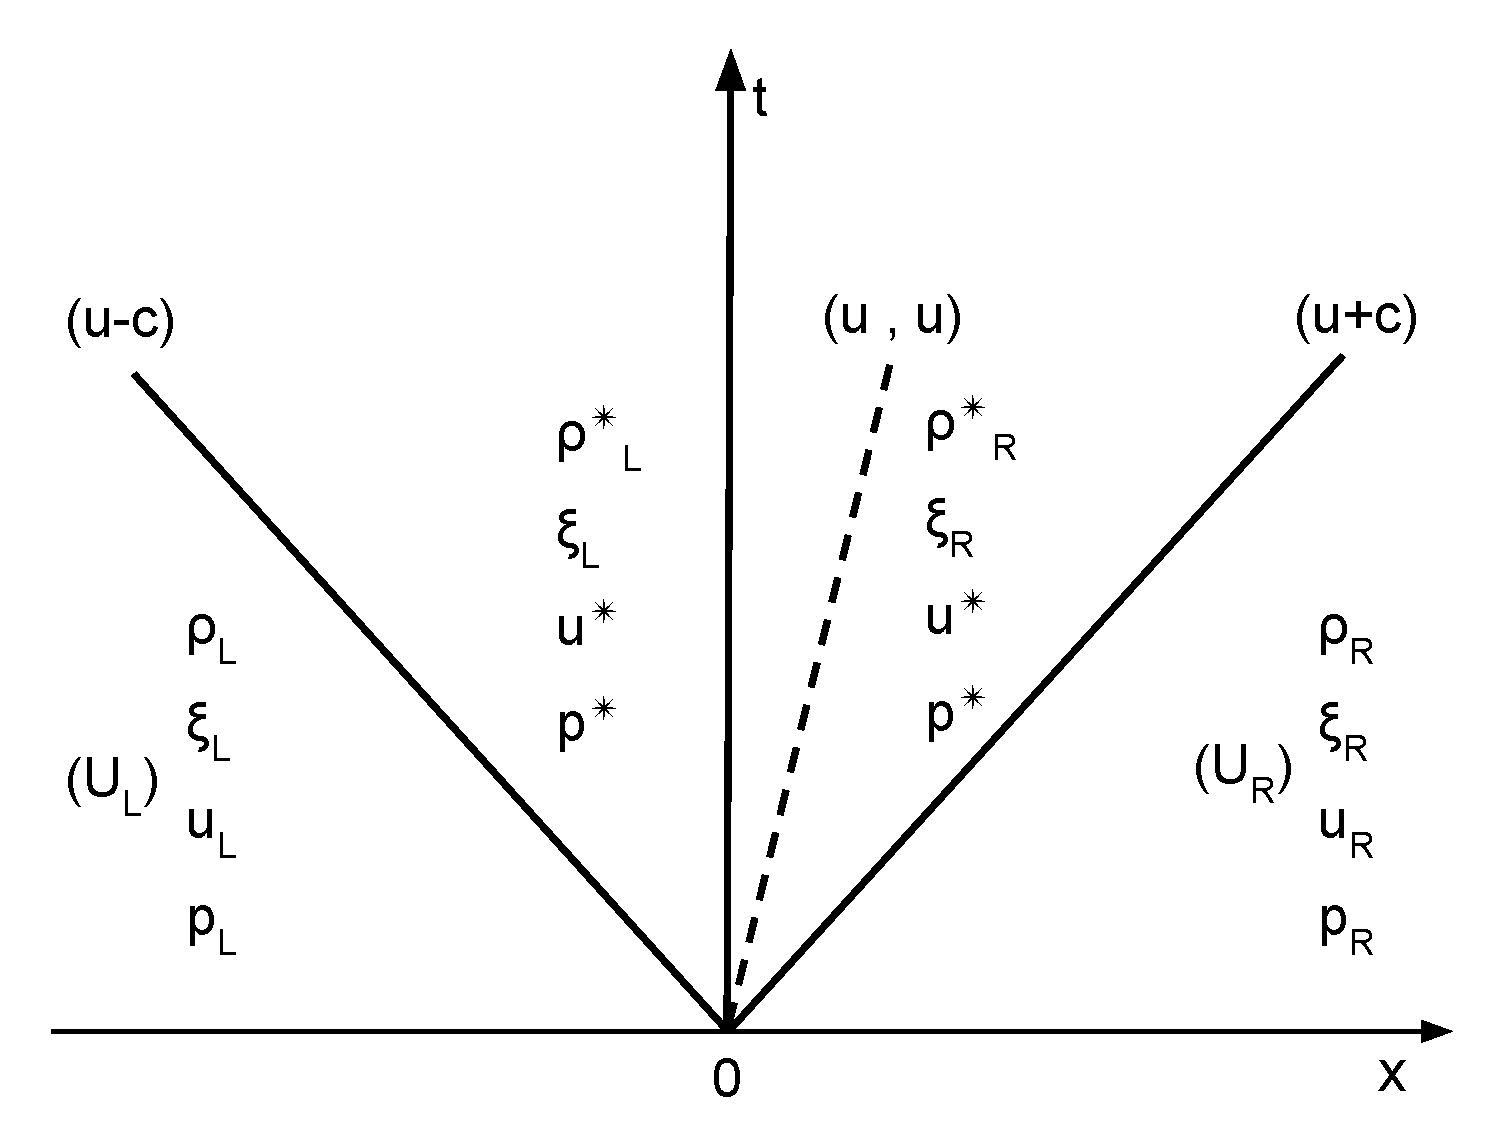
\includegraphics[width=6cm]{Chapter-2/Figures/Solution_Structure_RP}
\caption{The solution structure of Riemann problem for Plume-SPH governing equations}
\label{fig:Solution_Structure_RP}
\end{figure}
Based on the analysis on elementary wave solution for single waves, we get the structure of the solution of Riemann problem for system of governing equations as shown in Fig \ref{fig:Solution_Structure_RP}. The solution of mass fraction $\xi$ can be obtained separately from solving of other equations.
\begin{equation}
\xi =  \begin{cases} 
      \xi_L & x< ut\\
      \xi_R & x > ut
\end{cases}
\label{eq:RP_solution_xi}
\end{equation}
Since the solution of $\xi$ is independent of types of non-linear waves propagating left and right. $\xi$ can be updated separately before solving Riemann problems. This is easy to implement in discretized governing equations. The same discretized formulations (Eq. (\ref{eq:gov-sph-xi})) can be used to update mass fraction in GSPH.
\begin{figure}
\center
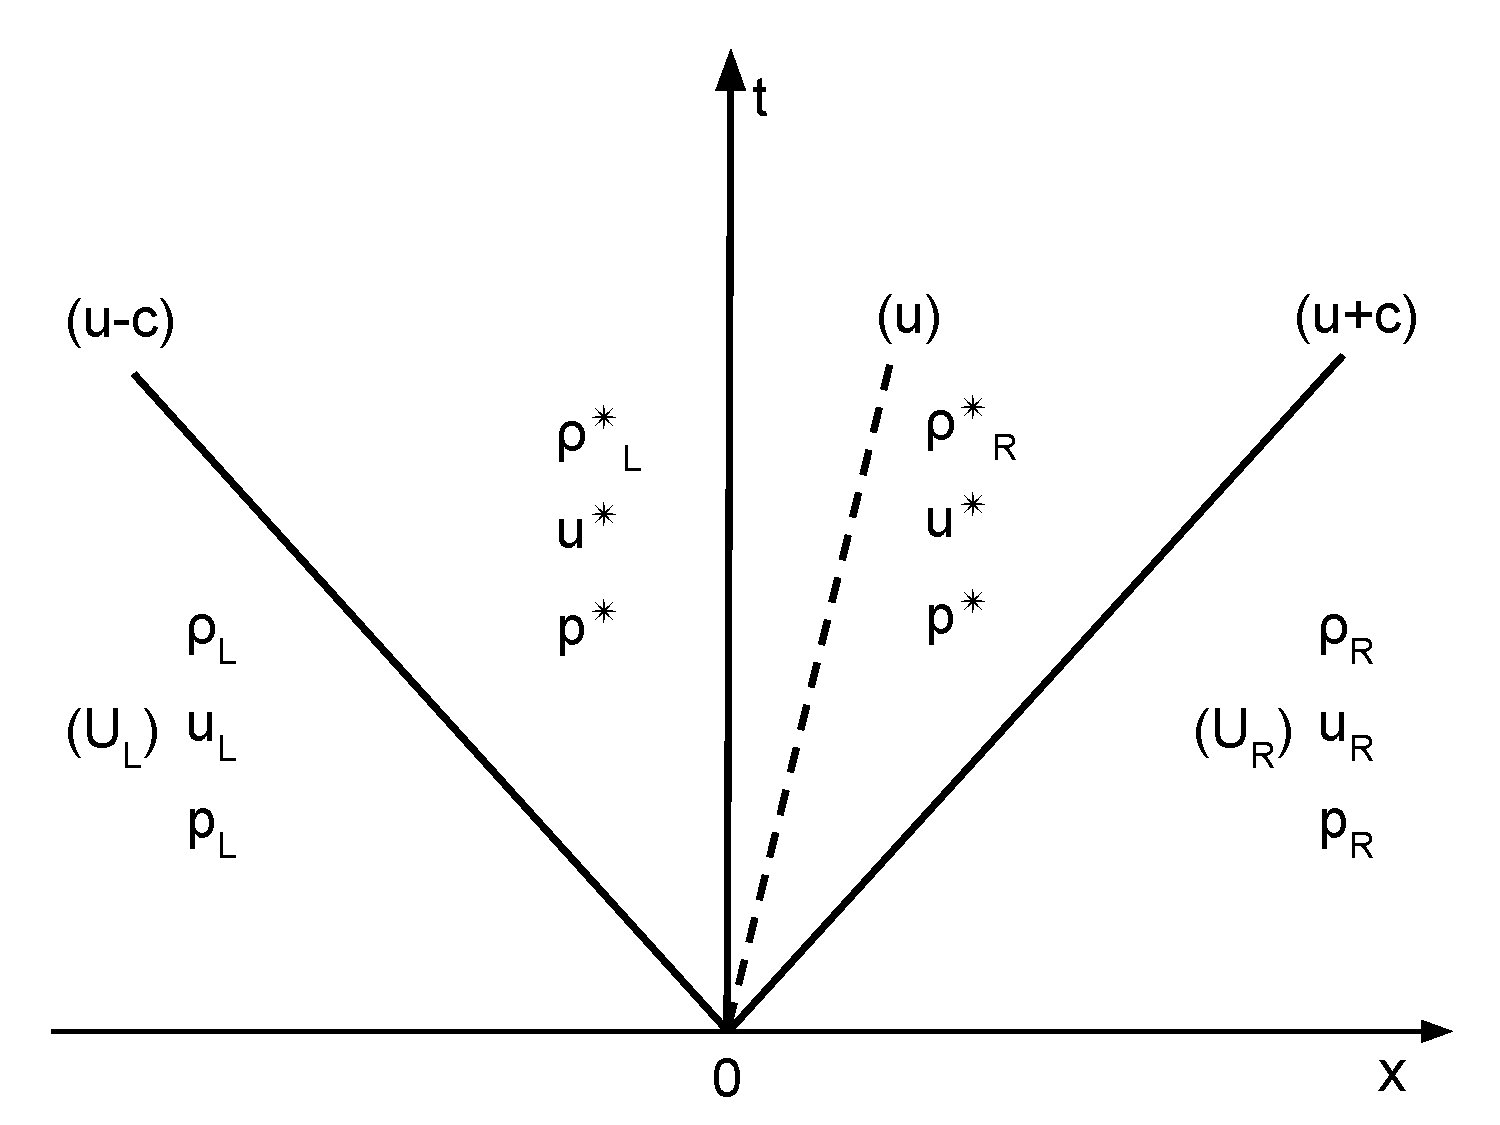
\includegraphics[width=6cm]{Chapter-2/Figures/Solution_Structure_RP_simplified}
\caption{The simplified solution structure of Riemann problems for Plume-SPH governing equations. The simplified solution structure is the same as that for Euler equation.}
\label{fig:Solution_Structure_RP_simplified}
\end{figure}
As the second equation in the original governing equations (Eq. (\ref{eq:gov-cs-rho}) $\sim$ (\ref{eq:gov-cs-e})) are weakly coupled with others and can be solved separately within each time step. Then remove Eq. (\ref{eq:gov-cs-ks}) from the original governing equations, the left will become Euler Equations. Equation (\ref{eq:gov-cs-rho}), (\ref{eq:gov-cs-v}), (\ref{eq:gov-cs-e}) together with Eq. (\ref{eq:EOS}) will form a complete system of equations with a space and time dependent $\gamma_{m}$. The solution structure of Riemann problems can be simplified as shown in Fig. \ref{fig:Solution_Structure_RP_simplified}, which is exactly the same as solution structure for Euler equations. It greatly simplifies the problem as there are plenty of (exact and approximate) Riemann solvers for Euler equations ready to use. Equation (\ref{eq:gov-nc-ks}) together with other equations, Eq. (\ref{eq:gov-gm}) - Eq. (\ref{eq:gov-ns}) will only be used to updating $\gamma_{m}$ which is a function of $\xi$. It is a separate procedure to update $\xi$ in SPH. Based on above analysis, it can be also a separate one in GSPH. In this way, equations are divided into two relatively independent groups, one represents Euler equations and the other one for updating $\gamma_{m}$.
The GSPH formulism \citep{inutsuka2002reformulation} proposed for sovling Euler equations can be directly used. In this case, we can use usual Riemann solvers for ideal gas (with a time and space dependent $\gamma$). Input variables for Riemann solvers will be $\rho=\rho^a + \rho^{sg}$, prssure $p$ and velocity $\textbf{v}$.
 
The only trick is, in this case, the specific heat ratio $\gamma_{m}$ is not a constant in space and time. Usually exact Riemann solvers for ideal gas are developed based on constant $\gamma_{m}$ assumptions. And an exact Riemann solver for not-constant gamma need to be driven in that case. Some numerical trick can be used. For example, when calculate $p^{ast}$ for the pair of two particles $\alpha$ and $\beta$, We can use Riemann solvers for a constant $\gamma_{m}=\frac{\gamma_{m,\alpha}+\gamma_{m,\beta}}{2}$.
Numerically, this treatment is sufficient. 